%% LyX 2.0.8.1 created this file.  For more info, see http://www.lyx.org/.
%% Do not edit unless you really know what you are doing.
\documentclass[10pt,serif]{beamer}
\usepackage[latin9]{inputenc}
\setcounter{secnumdepth}{3}
\setcounter{tocdepth}{3}
\setlength{\parskip}{0bp}
\setlength{\parindent}{0pt}
\definecolor{note_fontcolor}{rgb}{0.80078125, 0.80078125, 0.80078125}
\usepackage{array}
\usepackage{mathrsfs}
\usepackage{url}
\usepackage{bm}
\usepackage{amsmath}
\usepackage{amssymb}
\usepackage{mathdots}
\usepackage{graphicx}
\PassOptionsToPackage{version=3}{mhchem}
\usepackage{mhchem}
\usepackage{esint}
\usepackage[authoryear]{natbib}

\makeatletter

%%%%%%%%%%%%%%%%%%%%%%%%%%%%%% LyX specific LaTeX commands.
%% Because html converters don't know tabularnewline
\providecommand{\tabularnewline}{\\}
%% The greyedout annotation environment
\newenvironment{lyxgreyedout}
  {\textcolor{note_fontcolor}\bgroup\ignorespaces}
  {\ignorespacesafterend\egroup}
%% A simple dot to overcome graphicx limitations
\newcommand{\lyxdot}{.}


%%%%%%%%%%%%%%%%%%%%%%%%%%%%%% Textclass specific LaTeX commands.
 % this default might be overridden by plain title style
 \newcommand\makebeamertitle{\frame{\maketitle}}%
 \AtBeginDocument{
   \let\origtableofcontents=\tableofcontents
   \def\tableofcontents{\@ifnextchar[{\origtableofcontents}{\gobbletableofcontents}}
   \def\gobbletableofcontents#1{\origtableofcontents}
 }
 \def\lyxframeend{} % In case there is a superfluous frame end
 \long\def\lyxframe#1{\@lyxframe#1\@lyxframestop}%
 \def\@lyxframe{\@ifnextchar<{\@@lyxframe}{\@@lyxframe<*>}}%
 \def\@@lyxframe<#1>{\@ifnextchar[{\@@@lyxframe<#1>}{\@@@lyxframe<#1>[]}}
 \def\@@@lyxframe<#1>[{\@ifnextchar<{\@@@@@lyxframe<#1>[}{\@@@@lyxframe<#1>[<*>][}}
 \def\@@@@@lyxframe<#1>[#2]{\@ifnextchar[{\@@@@lyxframe<#1>[#2]}{\@@@@lyxframe<#1>[#2][]}}
 \long\def\@@@@lyxframe<#1>[#2][#3]#4\@lyxframestop#5\lyxframeend{%
   \frame<#1>[#2][#3]{\frametitle{#4}#5}}

%%%%%%%%%%%%%%%%%%%%%%%%%%%%%% User specified LaTeX commands.
\usepackage{animate}

% hack to get natbib working with beamer
\renewcommand{\newblock}{}

% list modifications
\setlength{\leftmargini}{0em}
\setlength{\leftmarginii}{1em}

% make $\times$, $+$, $-$ and $=$ use less space
\newcommand{\tims}{\negthinspace \times \negthinspace}
\newcommand{\eq}{\negthinspace = \negthinspace}
\newcommand{\plus}{\negthinspace + \negthinspace}
\newcommand{\minus}{\text{-}}
\newcommand{\smallcdot}{\negthinspace \cdot \negthinspace}

\newcommand{\nicefrac}[2]{\ensuremath ^{#1}\!\!/\!_{#2}}
\newcommand{\half}{\nicefrac{1}{2}}
\usepackage { fancybox}

\setlength{\tabcolsep}{2pt}

\makeatother

\begin{document}

\title{\vspace{-1.5cm}
\\
Optimal Transport and Mesh Adaptivity for Global Atmospheric Modelling\vspace{-0.5cm}
}


\author{Hilary Weller {\footnotesize{}(Meteorology, University of Reading)}
and \\
Phil Browne {\footnotesize{}(now at ECMWF)}}


\date{\vspace{-1cm}
\begin{tabular}{>{\centering}p{0.33\textwidth}>{\centering}p{0.33\textwidth}>{\centering}p{0.33\textwidth}}
 & 10 February 2017 & \includegraphics[scale=0.2]{/home/hilary/graphics/MetLogo}\tabularnewline
\end{tabular}}


\titlegraphic{%
\begin{tabular*}{1\textwidth}{@{\extracolsep{\fill}}l||r}
\multicolumn{2}{l}{\includegraphics[width=1\textwidth]{/home/hilary/OpenFOAM/hilary-2\lyxdot 3\lyxdot 0/run/meshes/sphereMeshes/MongeAmpereFromPpt/6/movie/pptMesh6}\vspace{-2.5cm}
}\tabularnewline
\end{tabular*}}

\makebeamertitle

\lyxframeend{}


\lyxframeend{}\lyxframe{NICAM at 7km resolution}

\url{http://nicam.jp/hiki/?About+NICAM}

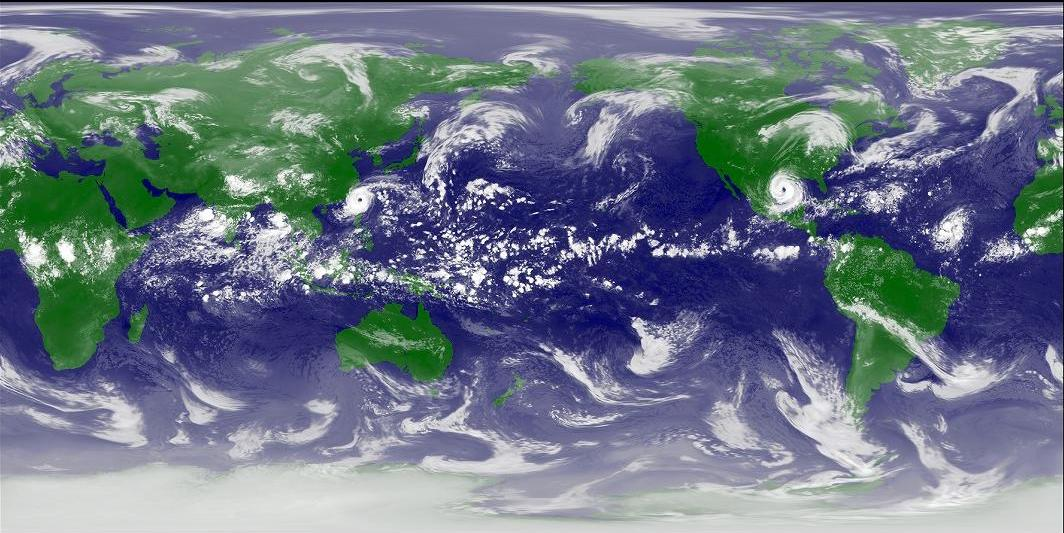
\includegraphics[width=1\textwidth]{graphics/nicam}


\lyxframeend{}


\lyxframeend{}\lyxframe{HadGEM at 25km resolution}

\url{https://hrcm.ceda.ac.uk/}

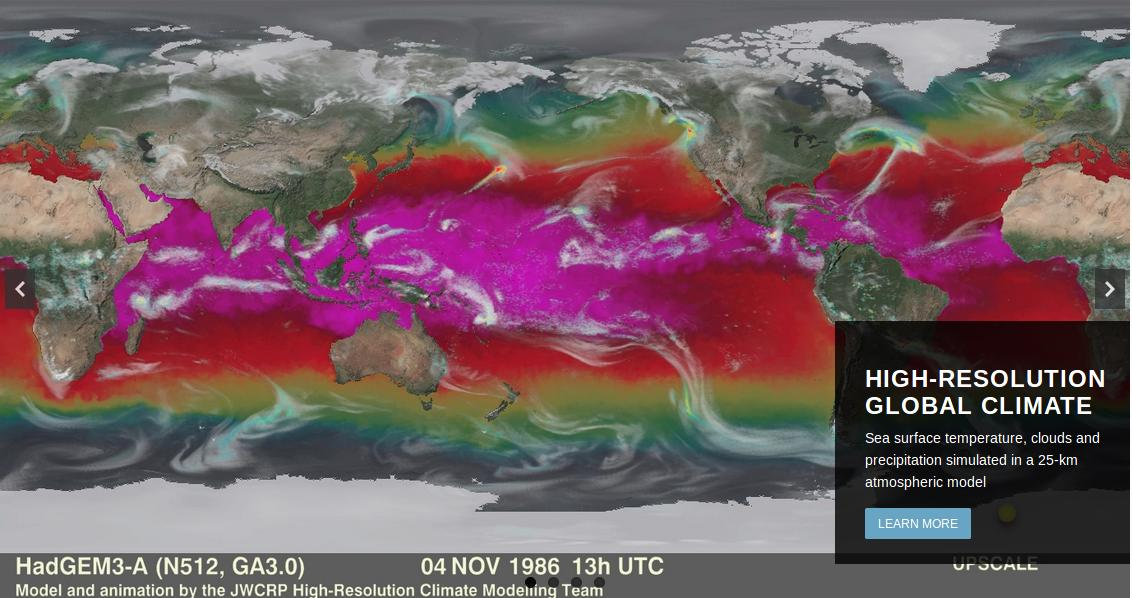
\includegraphics[width=1\textwidth]{graphics/hadgem}


\lyxframeend{}


\lyxframeend{}\lyxframe{Why Mesh Adaptivity?}
\begin{itemize}
\item High resolution needed to represent tropical precipitation
\item Too expensive 
\item Can local refinement help? \pause
\item Regional predictions of climate change
\end{itemize}
\includegraphics[width=0.75\textwidth]{graphics/pptChanges}

Precipitation changes under RCP 4.5 from CMIP5 multi-model mean. Hatching
where the multi-model mean change is less than the natural variability.
From \citet{XDV+15}


\lyxframeend{}


\lyxframeend{}\lyxframe{r-Adaptivity}
\begin{itemize}
\item \textbf{\textcolor{blue}{R}}edistribution, keeping mesh topology fixed
\item Deform mesh based on a monitor function
\item Why? \pause

\begin{itemize}
\item No load balancing problems\pause
\item No need to map solution between meshes\pause
\item Retro-fit to existing codes\pause
\end{itemize}
\item Who not?

\begin{itemize}
\item Distorted meshes
\item Never have complete control of $\Delta x$, $\Delta y$ and $\Delta z$
independently\pause
\end{itemize}
\end{itemize}

\lyxframeend{}


\lyxframeend{}\lyxframe{Shallow Water Flow Over a Mountain}

Relative Vorticity every 12 hours, fixed mesh of 10,242 hexagons FV
C-grid, local refinement of mountain ($\times2$):

\animategraphics[width=\linewidth,controls,poster=first]{3}{/home/hilary/OpenFOAM/hilary-2.3.0/run/shallowWaterSphere/WilliMountain/RinglerLloyd/6/2/movie/vorticity}{0}{30}


\lyxframeend{}


\lyxframeend{}\lyxframe{Shallow Water Flow Over a Mountain}

Relative Vorticity every 1 hour, fixed mesh of 10,242 hexagons FV
C-grid, local refinement of mountain ($\times2$):

\animategraphics[width=\linewidth,controls,poster=first]{3}{/home/hilary/OpenFOAM/hilary-2.3.0/run/shallowWaterSphere/WilliMountain/RinglerLloyd/6/2/movie/vort}{0}{24}


\lyxframeend{}


\lyxframeend{}\lyxframe{Shallow Water Flow Over a Mountain}

Mass divergence every 1 hours, fixed mesh of 10,242 hexagons FV C-grid,
local refinement of mountain ($\times2$):

\animategraphics[width=\linewidth,controls,poster=first]{3}{/home/hilary/OpenFOAM/hilary-2.3.0/run/shallowWaterSphere/WilliMountain/RinglerLloyd/6/2/movie/divhu}{0}{24}


\lyxframeend{}


\lyxframeend{}\lyxframe{Shallow Water Flow Over a Mountain}

Vorticity every 1 hour with h-adaptivity every 12 hours, mesh of 10,242
hexagons FV C-grid:

\animategraphics[width=\linewidth,controls,poster=first]{3}{/home/hilary/OpenFOAM/hilary-2.3.0/run/shallowWaterSphere/WilliMountain/adaptive/6_1_2_thicker/movie/vort}{0}{25}


\lyxframeend{}


\lyxframeend{}\lyxframe{Shallow Water Flow Over a Mountain}

Mass divergence every 1 hour with h-adaptivity every 12 hours, mesh
of 10,242 hexagons FV C-grid:

\animategraphics[width=\linewidth,controls,poster=first]{3}{/home/hilary/OpenFOAM/hilary-2.3.0/run/shallowWaterSphere/WilliMountain/adaptive/6_1_2_thicker/movie/divhu}{0}{25}


\lyxframeend{}


\lyxframeend{}\lyxframe{Might r-adaptivity help?}
\begin{itemize}
\item Solution evolves on a moving mesh

\begin{itemize}
\item solve equations relative to moving mesh
\item no mapping the solution between meshes
\item mesh changes every time-step
\end{itemize}
\item Refinement gradual in space and time \pause
\item First, how do we define the deforming mesh?
\end{itemize}

\lyxframeend{}


\lyxframeend{}\lyxframe{Optimally Transported Meshes in Euclidean Geometry }
\begin{itemize}
\item How to create a mesh which is equidistributed with respect to a monitor
function. ie
\[
A_{x}m\left(\mathbf{x}\right)=\text{const}
\]
 for each cell with area $A_{x}$ for mesh monitor function $m\left(\mathbf{x}\right)$.
\pause
\item Define a map from old mesh point, $\bm{\xi}$, to new mesh points,
$\mathbf{x}$ which is the gradient of a convex potential, $\phi$:
\[
\mathbf{x}=\bm{\xi}+\nabla\phi
\]
This leads to an \textbf{``optimally transported mesh''}, free of
tangling\pause
\item Jacobian determinant of mesh transform is the change in area:
\[
\det\left(\nabla\mathbf{x}\right)=A_{x}/A_{\xi}
\]

\item \pause Combine to form a Monge-Amp\'ere equation for mesh potential,
$\phi$:
\begin{eqnarray*}
\det\left(\nabla\left(\bm{\xi}+\nabla\phi\right)\right)m\left(\mathbf{x}\right) & = & \text{const}\\
\text{or }\ \det\left(I+H\left(\phi\right)\right) & = & \frac{\text{const}}{m\left(\mathbf{x}\right)}
\end{eqnarray*}

\item \pause This works fine in Euclidean geometry ...
\end{itemize}

\lyxframeend{}


\lyxframeend{}\lyxframe{Numerical Solution of the Monge-Amp�re Equation on a Plane \textmd{\normalsize{}(test
case from \citet{BRW15})}}

\begin{tabular}{ccc}
Monitor Function, $m$ & Initial Mesh & Solution of \tabularnewline
 &  & $|I+H\left(\phi\right)|m\left(\mathbf{x}\right)=\text{const}$\tabularnewline
\includegraphics[width=0.33\textwidth]{/home/hilary/OpenFOAM/hilary-2\lyxdot 3\lyxdot 0/run/meshes/plane/BuddRusselWalsh/Fig4\lyxdot 4_V0_moreDiags/1/monitor}\textrm{\pause} & \includegraphics[width=0.33\textwidth]{/home/hilary/OpenFOAM/hilary-2\lyxdot 3\lyxdot 0/run/meshes/plane/BuddRusselWalsh/blankCaseFig4\lyxdot 4_V0/constant/meshAll}\textrm{\pause} & \includegraphics[width=0.33\textwidth]{/home/hilary/OpenFOAM/hilary-2\lyxdot 3\lyxdot 0/run/meshes/plane/BuddRusselWalsh/Fig4\lyxdot 4_V0_moreDiags/1/Phi}\tabularnewline
\end{tabular}

Finite volume discretisation in space

Fixed point (Poincar�) outer iterations


\lyxframeend{}


\lyxframeend{}\lyxframe{Initial Mesh + $\nabla\phi$ gives an equidistributed mesh}

\begin{tabular}{ccc}
Initial Mesh, $\bm{\xi}$ & $+\nabla\phi$ & =$\mathbf{x}$\tabularnewline
\includegraphics[width=0.33\textwidth]{/home/hilary/OpenFOAM/hilary-2\lyxdot 3\lyxdot 0/run/meshes/plane/BuddRusselWalsh/blankCaseFig4\lyxdot 4_V0/constant/meshAll}\textrm{\pause} & \includegraphics[width=0.33\textwidth]{/home/hilary/OpenFOAM/hilary-2\lyxdot 3\lyxdot 0/run/meshes/plane/BuddRusselWalsh/Fig4\lyxdot 4_V0_moreDiags/1/Phi}\textrm{\pause} & \includegraphics[width=0.33\textwidth]{/home/hilary/OpenFOAM/hilary-2\lyxdot 3\lyxdot 0/run/meshes/plane/BuddRusselWalsh/Fig4\lyxdot 4_V0_moreDiags/1/meshAll}\tabularnewline
\end{tabular}


\lyxframeend{}\lyxframe{But on the Surface of a Sphere}
\begin{itemize}
\item The gradient of a potential does not map to point on the sphere
\item $\det\left(\nabla\nabla\phi\right)$ does not give change in area
\item $\therefore$ cannot formulate a Monge-Amp�re equation for the mesh
potential.
\end{itemize}
Instead:\pause
\begin{itemize}
\item Use exponential maps to map from old to new mesh:
\[
\mathbf{x}=\bm{\xi}+\exp_{\xi}\nabla\phi
\]

\item \textrm{\pause}Solve the optimal transport problem more directly...:
\begin{equation}
\frac{A_{x}}{A_{\xi}}=\frac{\text{const}}{m\left(\mathbf{x}\right)}\label{eq:MAsphere}
\end{equation}

\item \textrm{\pause }Linearise (\ref{eq:MAsphere}) about zero (assuming
tangent plane):
\[
\frac{A_{x}}{A_{\xi}}\approx\det\left(I+H\left(\phi\right)\right)\approx\pause1+\nabla^{2}\phi
\]

\item \textrm{\pause }Create Poincar� iterations with non-linear terms
treated explicitly:
\[
1+\nabla^{2}\phi^{n+1}=1+\nabla^{2}\phi^{n}-\frac{A_{x}}{A_{\xi}}+\frac{\text{const}^{n}}{m\left(\mathbf{x}^{n}\right)}
\]

\end{itemize}

\lyxframeend{}\lyxframe{An Optimally Transported Mesh}

Given the monitor function on the sphere:

\includegraphics[width=1\textwidth]{/home/hilary/OpenFOAM/hilary-2\lyxdot 3\lyxdot 0/run/meshes/sphereMeshes/MongeAmpereV1MedStencil/4/8/0/monitor}


\lyxframeend{}


\lyxframeend{}\lyxframe{An Optimally Transported Mesh}

The optimally transported mesh is calculated iteratively:

\animategraphics[width=\linewidth,controls,every=2,poster=first]{3}{/home/hilary/OpenFOAM/hilary-2.3.0/run/meshes/sphereMeshes/MongeAmpereV1MedStencil/4/8anim/movie/mesh}{0}{100}


\lyxframeend{}


\lyxframeend{}\lyxframe{Precipitation as a Monitor Function}

\vspace{-10pt}


{\footnotesize{}
\[
m=\frac{p+p_{\min}}{p_{\max}+p_{min}}\ \text{where}\ p_{\min}=10^{-5}\text{kg}\text{m}^{-2}\text{s}^{-1},\ p_{\max}=8.73\times10^{-4}\text{kg}\text{m}^{-2}\text{s}^{-1}
\]
}{\footnotesize \par}

\animategraphics[width=\linewidth,controls,poster=first,loop]{1}{/home/hilary/OpenFOAM/hilary-2.3.0/run/meshes/sphereMeshes/MongeAmpereFromPpt/6/movie/pptMesh}{0}{11}

{\small{}Using daily average precipitation rate, 1-12 Oct 2012, from
the NOAA-CIRES 20th Century Reanalysis version 2 (Compo et al, 2011,
\url{http://www.esrl.noaa.gov/psd/data/gridded/data.20thC_ReanV2.html})\vfill{}
See \citet*{WBBC16} }{\small \par}


\lyxframeend{}


\lyxframeend{}\lyxframe{Convergence is slow}
\begin{itemize}
\item We need to use a Newton solver rather than Poincar� iterations.
\item So we need to solve a PDE rather than a geometric equation
\item Need to linearise about previous iteration rather than about zero
\end{itemize}

\lyxframeend{}\lyxframe{Iterative Techniques for the Monge-Amp\'ere Equation}
\begin{itemize}
\item On the sphere we have used \textit{\textcolor{red}{Poincar\textit{\textcolor{red}{\'e}}
iterations}} with relaxation, $\alpha>1$:
\[
\alpha\nabla^{2}\phi^{\left(n+1\right)}=\alpha\nabla^{2}\phi^{\left(n\right)}-\frac{A_{x}}{A_{\xi}}+\frac{\text{const}^{n}}{m\left(\mathbf{x}^{n}\right)}
\]

\item \pause  \citet{BW06} proposed solving a\textit{\textcolor{red}{{}
Parabolic Monge-Amp\'ere Equation}}:
\[
\frac{\partial\phi}{\partial t}-\gamma\frac{\partial\nabla^{2}\phi}{\partial t}=\left(\det\left(I+H\left(\phi\right)\right)m\left(\mathbf{x}\right)\right)^{1/d}
\]

\end{itemize}
I will also describe\pause
\begin{enumerate}
\item A \textit{\textcolor{red}{Newton method }}\textcolor{black}{but only
with linearisation of $\det\left(I+H\left(\phi\right)\right)$}
\item A \textit{\textcolor{red}{Newton method }}\textcolor{black}{with linearisation
for $\det\left(I+H\left(\phi\right)\right)$ and $m\left(\mathbf{x}\right)$}
\end{enumerate}
In Euclidean Geometry


\lyxframeend{}


\lyxframeend{}\lyxframe{Newton 1, linearisation of \textcolor{black}{$\det\left(I+H\left(\phi\right)\right)$}}
\begin{itemize}
\item For the fixed-point iterations, we used $\det\left(I+H(\phi)\right)\approx1+\nabla^{2}\phi$
which was derived by linearising about $\phi=0$. \pause
\item Instead linearise about the previous iteration
\[
\phi^{n+1}\approx\phi^{n}+\phi^{\prime}
\]
\pause which gives:\hspace{2cm}$\det\left(I+H(\phi^{n+1})\right)\approx\det\left(I+H(\phi^{n})\right)+\nabla\cdot A^{n}\nabla\phi^{\prime}$\\
where $A^{n}=\left(\begin{array}{cc}
1+\phi_{yy}^{n} & -\phi_{xy}^{n}\\
-\phi_{xy}^{n} & 1+\phi_{xx}^{n}
\end{array}\right)$ in 2D Euclidean geometry.\pause 
\item So instead we solve for $\phi^{\prime}$ and the fixed-point iterations
become:
\[
\nabla\cdot A^{n}\nabla\phi^{\prime}=-\det\left(I+H(\phi^{n})\right)+\frac{\text{const}^{n}}{m(\mathbf{x}^{n})}
\]

\item \pause  To ensure that this equation remains elliptic, we may need
to modify $A$ to force it to be definite (all positive eigenvalues):
\[
B^{n}=A^{n}+\gamma I\ \text{ where }\ \gamma=\begin{cases}
0 & \text{ if }\min\sigma[A^{n}]>0\\
\varepsilon-\min\sigma[A^{n}] & \text{ if }\min\sigma[A^{n}]\le0
\end{cases}
\]

\end{itemize}

\lyxframeend{}\lyxframe{Full Newton Solver}
\begin{itemize}
\item The partial Newton solver iterations are:
\begin{equation}
\nabla\cdot A^{n}\nabla\phi^{\prime}=-\det\left(I+H(\phi^{n})\right)+\frac{\text{const}}{m(\mathbf{x})}\label{eq:AFP}
\end{equation}

\item \pause Also need to linearise $\frac{c}{m(\mathbf{x})}$:
\begin{eqnarray*}
\frac{c}{m}\left(\mathbf{x}^{n+1}\right) & \approx & \frac{c}{m}\left(\mathbf{x}^{n}\right)+\nabla_{x}\left(\frac{c}{m}\left(\mathbf{x}^{n}\right)\right)\cdot\left(\mathbf{x}^{n+1}-\mathbf{x}^{n}\right)\\
 & = & \frac{c}{m}\left(\mathbf{x}^{n}\right)+\nabla_{x}\left(\frac{c}{m}\left(\mathbf{x}^{n}\right)\right)\cdot\nabla\phi^{\prime}
\end{eqnarray*}

\item \pause Substituting into eqn(\ref{eq:AFP}) gives
\begin{equation}
\nabla\cdot A^{n}\nabla\phi^{\prime}=-\det\left(I+H(\phi^{n})\right)+\frac{c}{m}\left(\mathbf{x}^{n}\right)+\nabla_{x}\left(\frac{c}{m}\left(\mathbf{x}^{n}\right)\right)\cdot\nabla\phi^{\prime}\label{eq:Newton}
\end{equation}
\textrm{which is like an advection-diffusion equation for $\phi^{\prime}$
with tensorial diffusion $A^{n}$ and advecting velocity $\nabla_{x}\left(\frac{c}{m}\left(\mathbf{x}^{n}\right)\right)$.}\pause
\item Eqn (\ref{eq:Newton}) is a linear equation for $\phi^{\prime}$ which
is straightforward to solve (after spatial discretisation)
\end{itemize}

\lyxframeend{}


\lyxframeend{}\lyxframe{Results for the Ring Mesh}

Number of Iterations to Convergence (measured by variance of equidistribution,
$m|I+H(\phi)|$ )

\includegraphics[width=1\textwidth]{/home/hilary/Dropbox/PhilHilary/MA_iterative_images/equi_vs_iter_ring_PMA_Newt}


\lyxframeend{}


\lyxframeend{}\lyxframe{Results for the Ring Mesh}

Number of Iterations to Convergence (measured by variance of equidistribution,
$m|I+H(\phi)|$ )

\includegraphics[width=1\textwidth]{/home/hilary/Dropbox/PhilHilary/MA_iterative_images/equi_vs_iter_ring_FP_Newt}


\lyxframeend{}


\lyxframeend{}\lyxframe{Results for the Bell Mesh}

Number of Iterations to Convergence (measured by variance of equidistribution,
$m|I+H(\phi)|$ )

\includegraphics[width=1\textwidth]{/home/hilary/Dropbox/PhilHilary/MA_iterative_images/equi_vs_iter_bell_PMA_Newt}


\lyxframeend{}


\lyxframeend{}\lyxframe{Results for the Bell Mesh}

Number of Iterations to Convergence (measured by variance of equidistribution,
$m|I+H(\phi)|$ )

\includegraphics[width=1\textwidth]{/home/hilary/Dropbox/PhilHilary/MA_iterative_images/equi_vs_iter_bell_FP_Newt}


\lyxframeend{}


\lyxframeend{}\lyxframe{Scaling With Problem Size for the Ring}

\includegraphics[width=1\textwidth]{/home/hilary/Dropbox/PhilHilary/MA_iterative_images/tikz_scaling_ring_Newt}


\lyxframeend{}


\lyxframeend{}\lyxframe{Scaling With Problem Size for the Bell}

\includegraphics[width=1\textwidth]{/home/hilary/Dropbox/PhilHilary/MA_iterative_images/tikz_scaling_bell_Newt}


\lyxframeend{}


\lyxframeend{}\lyxframe{And on the sphere ...}


\lyxframeend{}\lyxframe{McRae's Monge-Amp�re like equation}

For optimal transport on a sphere \citep{MCB16}

\begin{equation}
m(\mathbf{x})\ \text{det}\left(\left(\nabla\exp\left(\nabla\phi\right)\bm{\xi}\right)\cdot P_{\xi}+\frac{\exp\left(\nabla\phi\right)\bm{\xi}}{R}\otimes\frac{\bm{\xi}}{R}\right)=\text{const}
\end{equation}


\begin{tabular}{>{\centering}p{0.13\textwidth}>{\raggedright}p{0.85\textwidth}}
$\bm{\xi}$ & Cartesian co-ordinates of a point on the sphere before the map\tabularnewline
$\mathbf{x}$ & Cartisian co-ordinates of the point on the sphere after the map\tabularnewline
$R$ & radius of the sphere\tabularnewline
$P_{\xi}$ & projection of the three-dimensional $\nabla\mathbf{x}$ onto the surface
of the sphere\tabularnewline
$\exp\left(\nabla\phi\right)$  &  exponential map which maps from $\bm{\xi}$ to $\mathbf{x}$ on the
sphere:\tabularnewline
\end{tabular}

\begin{equation}
\exp\left(\nabla\phi\right)\bm{\xi}=\cos\left(\frac{|\nabla\phi|}{R}\right)\bm{\xi}+R\sin\left(\frac{|\nabla\phi|}{R}\right)\frac{\nabla\phi}{|\nabla\phi|}
\end{equation}



\lyxframeend{}


\lyxframeend{}\lyxframe{Andrew McRae's solution}

Using mixed finite-elements in Firedrake \citep{MCB16}

\includegraphics[width=0.5\textwidth]{graphics/McRaeMAsolution}


\lyxframeend{}


\lyxframeend{}\lyxframe{Solving PDEs on Moving Meshes}


\lyxframeend{}\lyxframe{Solving PDEs on Moving Meshes}

\begin{minipage}[t]{0.7\columnwidth}%
Apply Reynolds transport theorem:
\[
\frac{d}{dt}\int_{\mathscr{V}(t)}\rho\ dV=\int_{\mathscr{V}(t)}\frac{\partial\rho}{\partial t}\ dV+\int_{S}\rho\ \mathbf{v}\cdot\mathbf{dS}
\]
to the continuity equation:
\begin{eqnarray*}
\frac{\partial\rho}{\partial t}+\nabla\cdot\left(\mathbf{u}\rho\right) & = & 0.
\end{eqnarray*}
Discretise in time and apply Gauss's divergence theorem:
\[
\frac{\mathscr{V}^{n+1}\rho^{n+1}-\mathscr{V}^{n}\rho^{n}}{\Delta t}=-\int_{S}\rho\left(\mathbf{u}-\mathbf{v}\right)\cdot\mathbf{dS}.
\]
%
\end{minipage}\hfill{} %
\begin{minipage}[t]{0.25\columnwidth}%
%
\noindent \begin{center}
\textbf{Definitions}:
\par\end{center}

\begin{tabular}{>{\raggedright}p{0.3\textwidth}>{\raggedright}p{1\textwidth}}
$\rho$ & %
density%
\tabularnewline
$\mathbf{u}$ & %
fluid velocity%
\tabularnewline
$\mathscr{V}(t)$ & %
cell volume%
\tabularnewline
$S(t)$ & %
cell surface%
\tabularnewline
$\mathbf{dS}$ & %
outward normal%
\tabularnewline
$\mathbf{v}$ & %
mesh velocity%
\tabularnewline
\multicolumn{2}{l}{%
\textrm{$\left(\mathbf{u}\!-\!\mathbf{v}\right)\cdot\mathbf{dS}$}%
}\tabularnewline
%
%
 & %
Volume flux%
\tabularnewline
\end{tabular}%
%
\end{minipage}


\lyxframeend{}


\lyxframeend{}\lyxframe{Discretisation}

\begin{minipage}[t]{0.48\columnwidth}%
%
\textbf{Definitions}:

\begin{tabular}{cl}
%
$n$%
 & %
Time-step number%
\tabularnewline
%
$\Delta t$%
 & %
Time-step%
\tabularnewline
%
$\rho^{\prime}$%
 & %
Temporary value of $\rho^{n+1}$%
\tabularnewline
%
$\phi_{r}$%
 & %
Relative face flux%
\tabularnewline
%
%
 & %
$=\left(\mathbf{u}\!-\!\mathbf{v}\right)\cdot\mathbf{dS}$%
\tabularnewline
\end{tabular}%
%
\end{minipage}\hfill{} %
\begin{minipage}[t]{0.48\columnwidth}%
%
\phantom{%
%
}\scalebox{0.5}[0.5]{\input{figs/twoCells.pdftex_t}}%
%
\end{minipage}
\begin{itemize}
\item Discretise in time using RK2:\pause 
\end{itemize}
\begin{eqnarray*}
\mathscr{V}_{f}^{n+1}\rho^{\prime} & = & \mathscr{V}_{f}^{n}\rho^{n}-\Delta t\left(\sum_{\text{faces}}\rho_{f}^{n}\phi_{r}\right)\\
\mathscr{V}_{f}^{n+1}\rho^{n+1} & = & \mathscr{V}_{f}^{n}\rho^{n}-\frac{\Delta t}{2}\left(\sum_{\text{faces}}\rho_{f}^{n}\phi_{r}+\sum_{\text{faces}}\rho_{f}^{\prime}\phi_{r}\right)
\end{eqnarray*}

\begin{itemize}
\item \pause Discretise in space using OpenFOAM's finite volume linear
upwind advection scheme.
\end{itemize}
\[
\rho_{f}=\rho_{u}+(\mathbf{x}_{f}-\mathbf{x}_{u})\cdot\nabla_{u}\rho
\]



\lyxframeend{}


\lyxframeend{}\lyxframe{Results - Solid body rotation}

Test case from \citet{LLM96}

$100\times100$ cells, 2,400 time-steps for one revolution

\begin{tabular}{>{\centering}p{0.48\textwidth}>{\centering}p{0.48\textwidth}}
Fixed Mesh & monitor $=\max\left(\frac{1}{16}+\frac{||\nabla\nabla\rho||}{3\times10^{-7}},1\right)$ \tabularnewline
\end{tabular}

\animategraphics[width=0.48\linewidth,controls,poster=first]{3}{/home/hilary/OpenFOAM/hilary-dev/AMMM/run/advection/solidBodyRotationOnPlane/uniformMesh/animategraphics/T_}{0}{12}
\animategraphics[width=0.48\linewidth,controls,poster=first]{3}{/home/hilary/OpenFOAM/hilary-dev/AMMM/run/advection/solidBodyRotationOnPlane/magGradTmonitor/animategraphics/T_}{0}{12}


\lyxframeend{}


\lyxframeend{}\lyxframe{Results - Solid body rotation}

Monitor function, monitor $=\max\left(\frac{1}{16}+\frac{||\nabla\nabla\rho||}{3\times10^{-7}},1\right)$
, is smoothed with Laplacian

\animategraphics[width=0.48\linewidth,controls,poster=first]{3}{/home/hilary/OpenFOAM/hilary-dev/AMMM/run/advection/solidBodyRotationOnPlane/magGradTmonitor/animategraphics/monitor_}{0}{12}
\animategraphics[width=0.48\linewidth,controls,poster=first]{3}{/home/hilary/OpenFOAM/hilary-dev/AMMM/run/advection/solidBodyRotationOnPlane/magGradTmonitor/animategraphics/mesh_}{0}{12}


\lyxframeend{}


\lyxframeend{}\lyxframe{Moving Meshes Over Mountains}


\lyxframeend{}\lyxframe{Advection Over a Mountain}

$100\times100$ cells, 2,400 time-steps for one revolution

Cone shaped mountain with peak height half the depth of the domain

\begin{tabular}{>{\centering}p{0.48\textwidth}>{\centering}p{0.48\textwidth}}
Fixed Mesh & monitor $=\max\left(\frac{1}{16}+\frac{||\nabla\nabla\rho||}{3\times10^{-7}},1\right)$ \tabularnewline
\end{tabular}

\animategraphics[width=0.48\linewidth,controls,poster=first]{3}{/home/hilary/OpenFOAM/hilary-dev/AMMM/run/advection/solidBodyRotationOnPlane/fixedMountain/animategraphics/T_}{0}{12}
\animategraphics[width=0.48\linewidth,controls,poster=first]{3}{/home/hilary/OpenFOAM/hilary-dev/AMMM/run/advection/solidBodyRotationOnPlane/magGradTmonitorMountainEmpty/animategraphics/T_}{0}{2}


\lyxframeend{}


\lyxframeend{}\lyxframe{Advection Over a Mountain with a Moving Mesh}

$100\times100$ cells, 2,400 time-steps for one revolution, monitor
$=\max\left(\frac{1}{16}+\frac{||\nabla\nabla\rho||}{3\times10^{-7}},1\right)$ 

Cone shaped mountain with peak height half the depth of the domain

\begin{tabular}{>{\centering}p{0.48\textwidth}>{\centering}p{0.48\textwidth}}
Mesh & Uniform tracer $\phi=\half$\tabularnewline
\end{tabular}

\animategraphics[width=0.48\linewidth,controls,poster=first]{3}{/home/hilary/OpenFOAM/hilary-dev/AMMM/run/advection/solidBodyRotationOnPlane/magGradTmonitorMountainEmpty/animategraphics/mesh_}{0}{2}
\animategraphics[width=0.48\linewidth,controls,poster=first]{3}{/home/hilary/OpenFOAM/hilary-dev/AMMM/run/advection/solidBodyRotationOnPlane/magGradTmonitorMountainEmpty/animategraphics/uniT_}{0}{2}


\lyxframeend{}


\lyxframeend{}\lyxframe{Advection Over a Mountain with a Moving Mesh}
\begin{itemize}
\item Zero relative flux over the ground
\item Mass of tracer conserved exactly ...\pause
\item Volume of the domain changes as the mesh moves over the mountain\pause


\noindent \textcolor{blue}{\Large{}Possible remedies}{\Large \par}

\item \pause Conservative mapping of old to new mesh

\begin{itemize}
\item Expensive
\item Exactly what we wanted to avoid with moving meshes
\item How to move vertices to get the desired volume\pause
\end{itemize}
\item An alternative

\begin{itemize}
\item Assume that the boundary condition is zero normal flow at the fixed
mountain surface
\item Calculate a relative flux as the mountain deforms \\
$\implies$ mass inside the domain will change in proportion to the
volume
\end{itemize}
\end{itemize}

\lyxframeend{}\lyxframe{With flow over the bottom boundary}

$100\times100$ cells, 2,400 time-steps for one revolution, monitor
$=\max\left(\frac{1}{16}+\frac{||\nabla\nabla\rho||}{3\times10^{-7}},1\right)$ 

Cone shaped mountain with peak height half the depth of the domain

Relative flux over the bottom boundary

\begin{tabular}{>{\centering}p{0.48\textwidth}>{\centering}p{0.48\textwidth}}
Gaussian tracer & Mesh\tabularnewline
\end{tabular}

\animategraphics[width=0.48\linewidth,controls,poster=first]{3}{/home/hilary/OpenFOAM/hilary-dev/AMMM/run/advection/solidBodyRotationOnPlane/magGradTmonitorMountain/animategraphics/T_}{0}{12}
\animategraphics[width=0.48\linewidth,controls,poster=first]{3}{/home/hilary/OpenFOAM/hilary-dev/AMMM/run/advection/solidBodyRotationOnPlane/magGradTmonitorMountain/animategraphics/mesh_}{0}{12}


\lyxframeend{}\lyxframe{With flow over the bottom boundary}

$100\times100$ cells, 2,400 time-steps for one revolution, monitor
$=\max\left(\frac{1}{16}+\frac{||\nabla\nabla\rho||}{3\times10^{-7}},1\right)$ 

Cone shaped mountain with peak height half the depth of the domain

Relative flux over the bottom boundary

\begin{tabular}{>{\centering}p{0.48\textwidth}>{\centering}p{0.48\textwidth}}
Uniform tracer $\phi=\half$ & \tabularnewline
\end{tabular}

\animategraphics[width=0.48\linewidth,controls,poster=first]{3}{/home/hilary/OpenFOAM/hilary-dev/AMMM/run/advection/solidBodyRotationOnPlane/magGradTmonitorMountain/animategraphics/uniT_}{0}{12}


\lyxframeend{}


\lyxframeend{}\lyxframe{Remaining Questions}
\begin{itemize}
\item Will this be stable when solving the Euler equation?
\item \pause What about conservative fluxes between bottom boundary and
domain

\begin{itemize}
\item air-sea fluxes
\end{itemize}
\item \pause What are the implications of the lack of mass conservation?
\item \pause How important is exact preservation of constants?
\end{itemize}

\lyxframeend{}\lyxframe{Hodge-dual C-grid with a moving mesh}

\begin{minipage}[t]{0.72\columnwidth}%
Shallow water equations in rotating frame in flux form:
\begin{eqnarray*}
\frac{\partial h\mathbf{u}}{\partial t}+\nabla\cdot\left(h\mathbf{u}\mathbf{u}\right) & = & -2h\bm{\Omega}\times\mathbf{u}-gh\nabla h\\
\frac{\partial h}{\partial t}+\nabla\cdot\left(h\mathbf{u}\right) & = & 0
\end{eqnarray*}
\scalebox{0.5}[0.5]{\input{/home/hilary/latex/codeDocumentation/movingShallowWaterH/figs/2dgeom.pdftex_t}}\hfill{}\scalebox{0.5}[0.5]{\input{/home/hilary/latex/codeDocumentation/movingShallowWaterH/figs/2dvars.pdftex_t}}%
\end{minipage}\hfill{} %
\begin{minipage}[t]{0.25\columnwidth}%
\noindent \begin{center}
\textbf{Definitions}:
\par\end{center}

%
\begin{tabular}{>{\raggedright}p{0.3\textwidth}>{\raggedright}p{1\textwidth}}
%
h%
 & %
fluid height%
\tabularnewline
%
$\mathbf{u}$%
 & %
fluid velocity%
\tabularnewline
%
$\bm{\Omega}$%
 & %
rotation%
\tabularnewline
%
$g$%
 & %
gravity%
\tabularnewline
%
$\mathbf{d}$%
 & %
vector between cell centres%
\tabularnewline
%
$V$%
 & %
$=h\mathbf{u}\cdot\mathbf{d}$%
\tabularnewline
%
%
 & %
prognostic%
\tabularnewline
%
$U$%
 & %
$=HV=h\mathbf{u}\cdot\mathbf{S}$%
\tabularnewline
%
%
 & %
mass flux%
\tabularnewline
\end{tabular}%
%
\end{minipage}


\lyxframeend{}\lyxframe{}

%
\begin{lyxgreyedout}
The shallow water height, $h$, is a prognostic variable located in
cells (at cell centres)

The moving mesh formulation starts with Reynolds transport theorem
for a field, $F$, over a domain, $\mathscr{V}(t)$ (a cell) with
boundary $S(t)$ (the cell faces):
\begin{equation}
\frac{d}{dt}\int_{\mathscr{V}(t)}F\ dV=\int_{\mathscr{V}(t)}\frac{\partial F}{\partial t}\ dV+\int_{S}F\ \mathbf{v}\cdot\mathbf{dS}\label{eq:ReynoldsTransport}
\end{equation}
where $\mathbf{v}$ is the velocity of the boundary and $\mathbf{dS}$
is the outward pointing normal to the boundary. The field $F$ can
be a scalar, vector or tensor field. We first consider the discretisation
of the full vector valued momentum equation over a control volume
with volume $\mathscr{V}^{n}$ (at time-level $n$), assume that $F=h\mathbf{u}$
and substitute the equation for $\partial h\mathbf{u}/\partial t$
from equation (\ref{eq:mom}) into equation (\ref{eq:ReynoldsTransport})
and discretise in time: 
\begin{equation}
\frac{\mathscr{V}^{n+1}h\mathbf{u}^{n+1}-\mathscr{V}^{n}h\mathbf{u}^{n}}{\Delta t}=-\int_{\mathscr{V}(t)}\nabla\cdot\left(h\mathbf{u}\mathbf{u}\right)+2h\bm{\Omega}\times\mathbf{u}+gh\nabla h\ dV+\int_{S}h\mathbf{u}\left(\mathbf{v}\cdot\mathbf{dS}\right)
\end{equation}
where $\Delta t$ is the time-step. Gauss's divergence theorem can
be applied to the advection term and this can then be combined with
the final term to give:
\begin{equation}
\frac{\mathscr{V}^{n+1}h\mathbf{u}^{n+1}-\mathscr{V}^{n}h\mathbf{u}^{n}}{\Delta t}=-\int_{S}h\mathbf{u}\left(\mathbf{u}-\mathbf{v}\right)\cdot\mathbf{dS}-\int_{\mathscr{V}(t)}2h\bm{\Omega}\times\mathbf{u}\ dV-\int_{\mathscr{V}(t)}gh\nabla h\ dV.\label{eq:momMoving}
\end{equation}
We define the velocity relative to the mesh face as
\begin{equation}
\mathbf{u}_{r}=\mathbf{u}-\mathbf{v}
\end{equation}
and the relative flux through the face as:
\begin{equation}
U_{r}=h\mathbf{u}_{r}\cdot\mathbf{S}.
\end{equation}
In order to solve the momentum equation on a moving C-grid (with a
Hodge operator) we solve the momentum equation in direction $\mathbf{d}^{n+1}$,
discretise in time using trapezoidal implicit and re-arrange the Coriolis
term so that the cross product can be pre-computed:
\begin{equation}
\frac{\mathscr{V}_{f}^{n+1}V^{n+1}-\mathscr{V}_{f}^{n}h\mathbf{u}^{n}\cdot\mathbf{d}^{n+1}}{\Delta t}=-\mathbf{d}^{n+1}\cdot\left(\sum_{\text{faces}}U_{r}\mathbf{u}\right)_{f}^{n+\half}-2\mathscr{V}_{f}(\mathbf{d}^{n+1}\times\bm{\Omega})\cdot(h\mathbf{u})^{n+\half}-\left(\mathscr{V}_{f}gh_{f}\nabla_{d}h\right)^{n+\half}\label{eq:momDotdMoving}
\end{equation}
where subscript $f$ means a field interpolated onto the face $f$.
The pressure gradient term is defined by $\nabla_{d}h=\mathbf{d}\cdot\nabla h$
so that the simplest discretisation of $\nabla_{d}h$ is simply the
difference between the two values of the height, $h$, either side
of the face. 

The diagnostic variable $h\mathbf{u}$ is reconstructed at faces from
surrounding values of $V$ following \citet{Wel14}. 

The advection and Coriolis terms are treated explicitly with deferred
correction of explicit terms, with parameter $\ell$ representing
values of variables at the most recent iteration within each time-step
but not at the latest time since they are not solved for implicitly.
The time-stepping can also include off-centering to improve stability,
with parameter $\alpha$: 
\begin{eqnarray}
\mathscr{V}_{f}^{n+1}V^{n+1} & = & \mathscr{V}_{f}^{n}h\mathbf{u}^{n}\cdot\mathbf{d}^{n+1}-(1-\alpha)\Delta t\left(\mathbf{d}^{n+1}\cdot\sum_{\text{faces}}\left(U_{r}\mathbf{u}\right)+2\mathscr{V}_{f}(\mathbf{d}^{n+1}\times\bm{\Omega})\cdot(h\mathbf{u})+\mathscr{V}_{f}gh_{f}\nabla_{d}h\right)^{n}\label{eq:momD}\\
 & - & \alpha\Delta t\left\{ \left(\nabla\cdot\left(U_{r}\mathbf{u}\right)^{\ell}\right)\cdot\mathbf{d}^{n+1}+2\mathscr{V}_{f}\left(\mathbf{d}^{n+1}\times\bm{\Omega}\right)_{f}\cdot(h\mathbf{u}^{\ell})+\mathscr{V}_{f}^{n+1}gh_{f}\nabla_{d}p^{n+1}\right\} .
\end{eqnarray}
Note that for the variables defined at time-level $n$, the volume
is defined at time-level $n$ but the direction, $d$, is defined
at time-level $n+1$ so that $ $$\left(\mathscr{V}_{f}\nabla_{d}h\right)^{n}=\mathscr{V}_{f}^{n}\mathbf{d}^{n+1}\cdot\nabla h^{n}$. 

Next we define an intermediate values, $V^{o}$ and $V^{\prime}$,
(which share the same storage as $V^{n}$ and $V^{n+1}$) using all
explicitly defined values:
\begin{eqnarray}
V^{o} & = & \left\{ \mathscr{V}_{f}^{n}h\mathbf{u}^{n}\cdot\mathbf{d}^{n+1}-(1-\alpha)\Delta t\left(\mathbf{d}^{n+1}\cdot\left(\sum_{f\in\text{faces}}U_{r}\mathbf{u}\right)_{f}+2\mathscr{V}_{f}(\mathbf{d}^{n+1}\times\bm{\Omega})\cdot\left(h\mathbf{u}\right)+\mathscr{V}_{f}gh_{f}\nabla_{d}h\right)^{n}\right\} \bigg/\mathscr{V}_{f}^{n+1}\label{eq:Vi}\\
V^{\prime} & = & V^{o}-\alpha\Delta t\mathbf{d}^{n+1}\cdot\left(\sum_{f\in\text{faces}}U_{r}\mathbf{u}\right)_{f}^{\ell}/\mathscr{V}_{f}^{n+1}
\end{eqnarray}
Variables $V$ and $V^{\prime}$ share the same boundary conditions
at zero flux boundaries (ie they are all set to zero at zero flux
boundaries). This is why the Coriolis term has not yet been added
to $V^{\prime}$ as it would violate the boundary conditions. Next
we apply the Hodge operator, $H$, add the Coriolis term and add the
non-orthogonal part of the pressure gradient to find the intermediate
value of the absolute flux, before the orthogonal part of the pressure
gradient is applied:
\begin{eqnarray}
U^{\prime} & = & HV^{\prime}-2\alpha\Delta t\ H\left(\left(\mathbf{d}^{n+1}\times\bm{\Omega}\right)\cdot(h\mathbf{u}^{\ell})\right)-\alpha\Delta t\ gH_{\text{off}}h_{f}^{\ell}\nabla_{d}h^{\ell}
\end{eqnarray}
After the numerical solution of the Helmholtz equation to find $h^{n+1}$,
we will be able to back-substitute to calculate $V^{n+1}$, $U^{n+1}$
and the relative flux, $U_{r}^{n+1}$:
\begin{eqnarray}
V^{n+1} & = & V^{\prime}-2\alpha\Delta t\ \left(\mathbf{d}^{n+1}\times\bm{\Omega}\right)\cdot(h\mathbf{u}^{\ell})-\alpha\Delta t\ gh_{f}^{\ell}\nabla_{d}h^{n+1}\label{eq:backSubsV}\\
U^{n+1} & = & U^{\prime}-\Delta t\alpha gH_{d}h_{f}\nabla_{d}h^{n+1}.\label{eq:backSubsFlux}\\
U_{r}^{n+1} & = & U^{n+1}-h_{f}^{n+\half}\mathbf{v}^{n+\half}\cdot\mathbf{S}.\label{eq:backSubsRelFlux}
\end{eqnarray}
We require the momentum, $h\mathbf{u}$, to satisfy the continuity
equation at every time-step. Applying the Reynolds transport theorem
(eqn \ref{eq:ReynoldsTransport}) to the continuity equation (\ref{eq:cont})
using $F=h$ and discretising in space and time gives:
\begin{equation}
\frac{\mathscr{V}_{f}^{n+1}h^{n+1}-\mathscr{V}_{f}^{n}h^{n}}{\Delta t}=-(1-\alpha)\sum_{\text{faces}}U_{r}^{n}-\alpha\sum_{\text{faces}}U_{r}^{n+1}.\label{eq:divU}
\end{equation}
The Helmholtz equation for $h^{n+1}$ can be formulated using eqns
(\ref{eq:backSubsV}-\ref{eq:backSubsRelFlux}):
\begin{equation}
\frac{\mathscr{V}_{f}^{n+1}h^{n+1}-\mathscr{V}_{f}^{n}h^{n}}{\Delta t}=\sum_{\text{faces}}h_{f}^{n+\half}\mathbf{v}\cdot S-\alpha\sum_{\text{faces}}U^{n}-(1-\alpha)\sum_{\text{faces}}U^{\prime}-\alpha^{2}\sum_{\text{faces}}\Delta tgH_{d}h_{f}\nabla_{d}h^{n+1}.\label{eq:p}
\end{equation}
This is a Helpholtz equation because the final term is a discretisation
of the Laplacian, $\nabla\cdot\left(gh\nabla h\right)$. In order
to simplify the construction of the matrix for the implicit solution
of (\ref{eq:p}), the Hodge operator, $H$ has been separated into
diagonal and off-diagonal parts:
\begin{eqnarray}
H\nabla_{d}h & = & H_{d}\nabla_{d}h+H_{\text{off}}\nabla_{d}h\\
 & = & \frac{|\mathbf{S}|}{|\mathbf{d}|}\nabla_{d}h+H_{\text{off}}\nabla_{d}h
\end{eqnarray}
and only solve the diagonal part implicitly.

Equation (\ref{eq:p}) is solved implicitly for $h^{n+1}$ and then
we can calculate momentum components, $U$ and $V$ (the back-substitution
step) using eqns (\ref{eq:backSubsV}) and (\ref{eq:backSubsFlux})
and then reconstruct $h\mathbf{u}$ at the faces.

In order to ensure no flow at boundaries, geostrophic balance can
be imposed, ie:
\begin{equation}
g\nabla_{n}h=-2\left(\bm{\Omega}\times\mathbf{u}\right)\cdot\mathbf{n}=-2\left(\mathbf{n}\times\bm{\Omega}\right)\cdot\mathbf{u}
\end{equation}
at boundaries where $\mathbf{n}$ is the outward pointing unit normal
at the boundary. %
\end{lyxgreyedout}


%

\lyxframeend{}\lyxframe{Results of Shallow Water Equations on a $\beta$ plane}

Vorticity of a barotropically unstable jet every $10^{5}$ seconds
$\sim28$ hours

$300\times100$ cells, fixed mesh

\animategraphics[width=\linewidth,controls,poster=first]{3}{/home/hilary/OpenFOAM/hilary-dev/AMMM/run/shallowWater/baroJet/uniformHiRes/animategraphics/vorticity_}{0}{10}


\lyxframeend{}\lyxframe{}

$150\times50$ cells, fixed mesh

\animategraphics[width=0.9\linewidth,controls,poster=first]{3}{/home/hilary/OpenFOAM/hilary-dev/AMMM/run/shallowWater/baroJet/uniformMesh/animategraphics/vorticity_}{0}{10}

$150\times50$ cells, r-adaptive, monitor $=\max\left(1/4+||\nabla\mathbf{u}||/2\times10^{-4},1\right)$ 

\animategraphics[width=0.9\linewidth,controls,poster=first]{3}{/home/hilary/OpenFOAM/hilary-dev/AMMM/run/shallowWater/baroJet/linGradU_3_smallerBump/animategraphics/vorticity_}{0}{10}


\lyxframeend{}\lyxframe{References}

\textcolor{black}{\tiny{}\bibliographystyle{plainnat}
\bibliography{numerics}
}{\tiny \par}


\lyxframeend{}
\end{document}
